%-------------------------------------------------------------
\subsection{Example 4} \label{sec:ch5:example4}

%-------------------------------------------------------------
\subsubsection{Description}

For the fourth example, we will consider the finite-horizon LQR problem in Prob.~(\ref{eq:ch5:lqr}) \cite{Bryson1975a,Liberzon2012a}:%
\begin{subequations}%%
\begin{align}
\min_{\bm{u}(t)} \quad & \left[ \bm{\xi}\tran \bm{M} \bm{\xi} \right]_{t=t_f} + 
\int_{t_0}^{t_f} \left[ \bm{\xi}\tran \bm{Q} \bm{\xi} + \bm{u}\tran \bm{R} \bm{u} \right] dt \\
\text{subject to:} \quad & \dot{\bm{\xi}} = \bm{A} \bm{\xi} + \bm{B} \bm{u} \\
& \bm{\xi}(t_0) = \bm{\xi}_0
\end{align}
\end{subequations}%

\noindent where $\bm{M}$ and $\bm{Q}$ are symmetric positive semidefinite and $\bm{R}$ is symmetric positive definite.
The structure-based problem description for this example is:%
\allowdisplaybreaks[1]%
\begin{subequations}%%
\begin{gather}
% Mayer term
\mathcal{M}\xind{1}.\xvar{left} = 5, \quad \mathcal{M}\xind{1}.\xvar{right} = 5, \quad \mathcal{M}\xind{1}.\xvar{matrix} = \bm{M} \\
% Lagrange term
\mathcal{L}\xind{1}.\xvar{left} = 2, \quad \mathcal{L}\xind{1}.\xvar{right} = 2, \quad \mathcal{L}\xind{1}.\xvar{matrix} = \bm{Q} \\
\mathcal{L}\xind{2}.\xvar{left} = 1, \quad \mathcal{L}\xind{2}.\xvar{right} = 1, \quad \mathcal{L}\xind{2}.\xvar{matrix} = \bm{R} \\
% dynamics
% \bm{A}, \bm{B} \text{ given} \\
% initial condition
\mathcal{UB}\xind{1}.\xvar{right} = 4, \quad \mathcal{UB}\xind{1}.\xvar{matrix} = \bm{\xi}_0, \quad
\mathcal{LB}\xind{1}.\xvar{right} = 4, \quad \mathcal{LB}\xind{1}.\xvar{matrix} = \bm{\xi}_0
\end{gather}
\end{subequations}%%
\allowdisplaybreaks[0]%

\noindent The \textsc{Matlab} code is in Sec.~\ref{sec:ex4-code}.

%-------------------------------------------------------------
\subsubsection{Solution} \label{sec:ch5:ex4:solution}

\begin{figure}
\centering

\begin{subfigure}{0.5\textwidth}
\centering
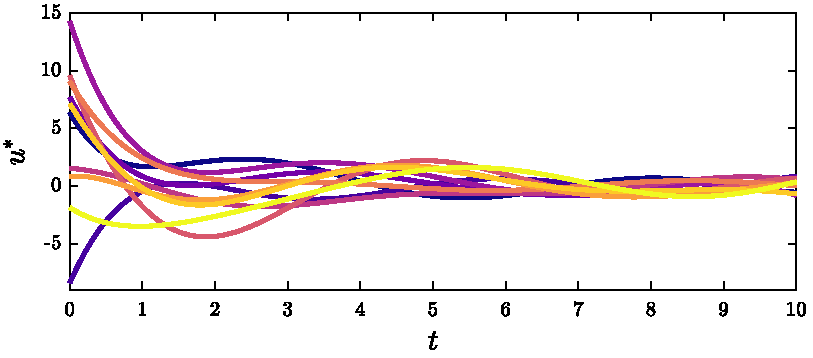
\includegraphics[width=\textwidth]{../ch5/figures/ex4sol-controls}%
\caption{Control.}
\label{fig:ch5:ex4sol:controls}
\end{subfigure}%
\begin{subfigure}{0.5\textwidth}
\centering
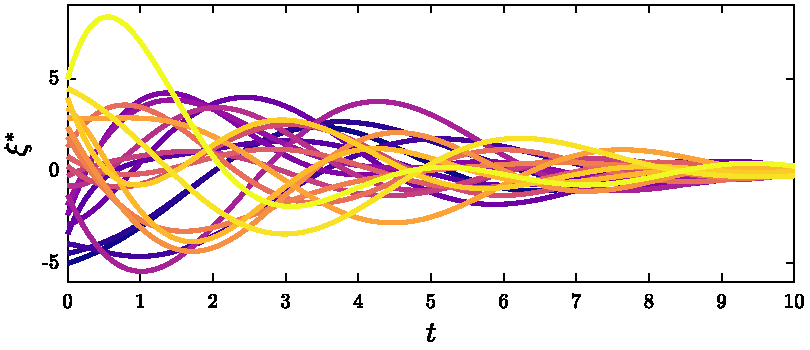
\includegraphics[width=\textwidth]{../ch5/figures/ex4sol-states}%
\caption{States.}
\label{fig:ch5:ex4sol:states}
\end{subfigure}%

\caption{Solution for \nameref{sec:ch5:example4}.}
\label{fig:ch5:ex4sol}
\end{figure}

The optimal control has the following form \cite{Bryson1975a,Liberzon2012a}:
\begin{align}
\bm{u}^* = - \bm{R}^{-1} \bm{B}\tran \bm{P} \bm{\xi}
\end{align}

\noindent where $\bm{P}$ is symmetric positive semidefinite matrix that is a solution to the following differential equation and boundary condition:
\begin{align}
\dot{\bm{P}} = -\bm{Q} - \bm{A}\tran \bm{P} - \bm{P} \bm{A} + \bm{P} \bm{B} \bm{R}^{-1} \bm{B}\tran \bm{P}, \quad \bm{P}(t_f) = \bm{M}
\end{align}

\noindent The specific problem parameters are shown in Sec.~\ref{sec:ex4-code} ($n_\xi = 20$ and $n_u=10$ with generated matrices).
The optimal trajectories for controls and states are shown in Fig.~\ref{fig:ch5:ex4sol}, and were determined by numerically solving the BVP problem with a relative error tolerance at $10^{-10}$.

%-------------------------------------------------------------
\subsubsection{Numerical results}

\begin{figure}%
\centering

{\footnotesize Local maximum values (local minimum values are in a thinner, translucent color):}


\includegraphics[width=\textwidth]{../ch5/figures/ex1_sens_legend}%

\vspace{1mm}

\begin{subfigure}{0.5\textwidth}
\centering
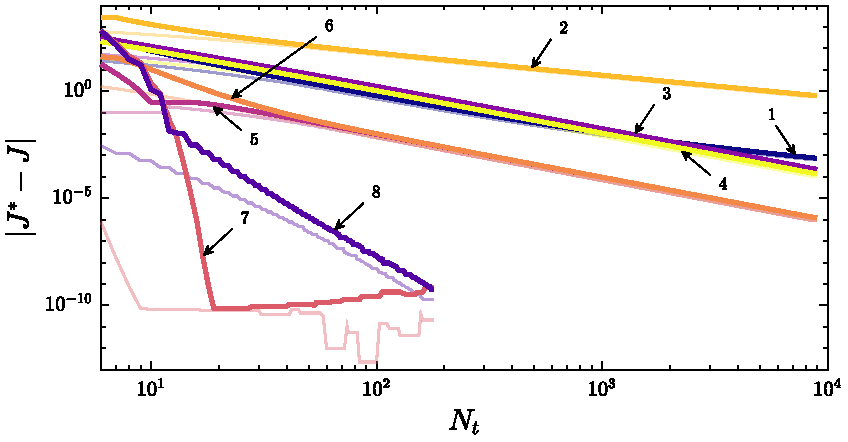
\includegraphics[width=\textwidth]{../ch5/figures/ex4_sens_objective}%
\caption{Objective error.}
\label{fig:ch5:ex4sens:objective}
\end{subfigure}%
\begin{subfigure}{0.5\textwidth}
\centering
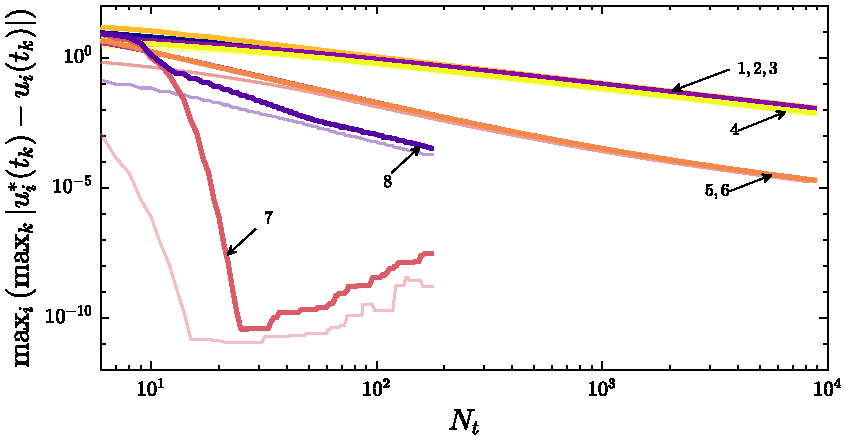
\includegraphics[width=\textwidth]{../ch5/figures/ex4_sens_control}%
\caption{Control error.}
\label{fig:ch5:ex4sens:control}
\end{subfigure}%

\begin{subfigure}{0.5\textwidth}
\centering
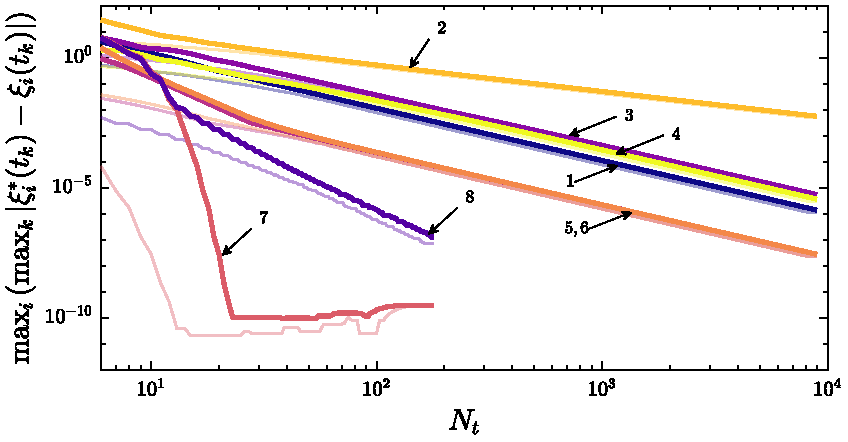
\includegraphics[width=\textwidth]{../ch5/figures/ex4_sens_state_1}%
\caption{State error.}
\label{fig:ch5:ex4sens:state-1}
\end{subfigure}%
\begin{subfigure}{0.5\textwidth}
\centering
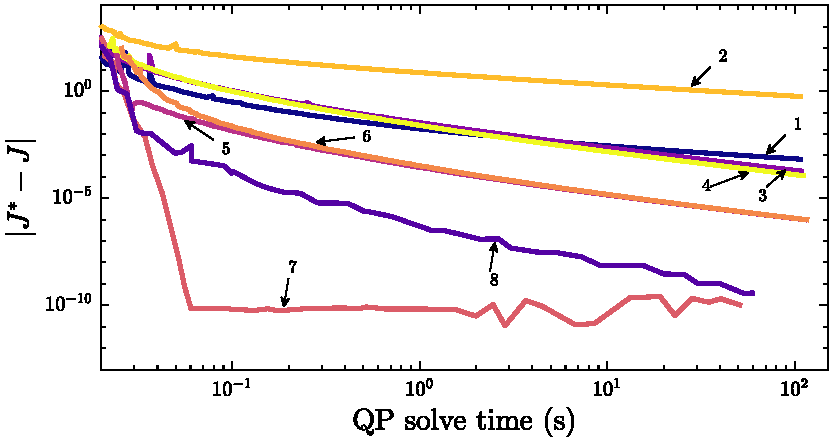
\includegraphics[width=\textwidth]{../ch5/figures/ex4_sens_solve_time}%
\caption{Objective error vs. total \qp{} solve time.}
\label{fig:ch5:ex4sens:solvetime}
\end{subfigure}%

\caption{Numerical results for \nameref{sec:ch5:example4}.}
\label{fig:ch5:ex4sens}
\end{figure}

The convergence results for the eight tested schemes are shown in Fig.~\ref{fig:ch5:ex4sens}.
The numerical results for this example are quite similar to \nameref{sec:ch5:example1} (see Fig.~\ref{fig:ch5:ex1sens}).
The PS-based methods (7,8) performed the best, followed by the CQHS-based methods (5,6). Then was (1,3,4) and finally (1) was the worst again.
The primary discussion point for this example is the efficiency at which the LQR problem was solved.
The objective error vs. total \qp{} solve time is shown in Fig.~\ref{fig:ch5:ex4sens:solvetime}.
LGL-PS-G (7) with $N_t=23$ took only 0.2~s to create and solve the \qp{} with an accuracy in states, controls, and objective value at the tolerance used ($10^{-10}$) when generating the BVP solution in Sec.~\ref{sec:ch5:ex4:solution}.
These results demonstrate that \dt{} approximations of the finite-horizon LQR problem can be a competitive solution strategy.